\PassOptionsToPackage{table}{xcolor}
% CAS loads legacy STIX math; XeTeX uses unicode-math below instead.
\ifdefined\XeTeXversion
\expandafter\def\csname ver@stix.sty\endcsname{2026/10/15}
\fi
\documentclass[a4paper,fleqn]{cas-sc}
\ifdefined\XeTeXversion
\usepackage{fontspec}
\setmainfont{texgyretermes-regular.otf}[BoldFont=texgyretermes-bold.otf,ItalicFont=texgyretermes-italic.otf,BoldItalicFont=texgyretermes-bolditalic.otf]
\setsansfont{texgyreheros-regular.otf}[BoldFont=texgyreheros-bold.otf,ItalicFont=texgyreheros-italic.otf]
\setmonofont{texgyrecursor-regular.otf}
\else
\usepackage[T5]{fontenc}
\usepackage[utf8]{inputenc}
\fi
\usepackage[vietnamese]{babel}
\usepackage[numbers]{natbib}
\usepackage{amsmath,amssymb,booktabs,longtable,tabularx,array}
\usepackage{graphicx,url,xcolor}
\usepackage{enumitem}
\ifdefined\XeTeXversion
\usepackage{unicode-math}
\setmathfont{texgyretermes-math.otf}
\providecommand{\square}{\mdlgwhtsquare}
\fi
\setlength{\emergencystretch}{3em}
\setlist{itemsep=2pt,topsep=4pt}
\newsavebox{\btlTableBox}
\newcommand{\FitTableWidth}[1]{%
\sbox{\btlTableBox}{#1}%
\ifdim\wd\btlTableBox>\linewidth
\resizebox{\linewidth}{!}{\usebox{\btlTableBox}}%
\else\usebox{\btlTableBox}\fi}
\renewcommand{\printorcid}{}
\ExplSyntaxOn
\cs_set:Npn \__first_footerline:
 {\small\sffamily Nguyễn~Duy~Trường:~\rmfamily\itshape Báo~cáo~bài~tập~lớn~số~1}
\ExplSyntaxOff
\graphicspath{{generated/}}
\begin{document}
\shorttitle{Mã hóa SAT cho N Queens}
\shortauthors{Nguyễn Duy Trường}
\title[mode=title]{Mã hóa SAT và so sánh các phương pháp giải chính xác cho bài toán N Queens}
\author[1]{Nguyễn Duy Trường}
\affiliation[1]{organization={Trường Đại học Công nghệ, Đại học Quốc gia Hà Nội},
city={Hà Nội},country={Việt Nam}}
\begin{abstract}
Báo cáo cài đặt và đánh giá năm mã hóa SAT cho bài toán N-Queens trên bàn cờ trống: pairwise, binary, sequential counter, commander đệ quy và product. Các mô hình dùng cùng ràng buộc hàng, cột, đường chéo; nghiệm được kiểm tra hình học độc lập. Tính đúng được đối chiếu qua 2555 phép gán AMO nhỏ, 60 trường hợp SAT/UNSAT và đếm nghiệm đến N=8. Tập chính gồm năm kích thước từ 8 đến 128, mỗi cấu hình lặp ba lần; tập mở rộng khảo sát N=256,512,1000 với hạn tổng 30 giây. Trên tập chính, SAT hoàn thành 63/75 lần chạy; binary nhanh hơn pairwise khoảng 3.69 lần ở N=64. Kết quả cho thấy giảm số clause không bảo đảm giảm thời gian giải, và không có encoding thắng trên mọi kích thước đã xét. Báo cáo đối chiếu với CP-SAT, CPLEX CP, CPLEX MIP và Gurobi trong miền giấy phép khả dụng, đồng thời công bố các giới hạn kích thước. Toàn bộ mã nguồn, dữ liệu đo và quy trình tái lập được cung cấp kèm báo cáo.
\end{abstract}
\begin{keywords}
N Queens \sep SAT solving \sep CNF encoding \sep cardinality constraints \sep constraint programming
\end{keywords}
\maketitle
\noindent\textbf{Bài tập lớn số 1.} Học phần Các vấn đề hiện đại trong KHMT,
HK I năm học 2026--2027. Mã sinh viên 24021650. Lớp CS5.
Email: \texttt{truong0816081519@gmail.com}.

% Phần lý thuyết của báo cáo. Ghép sau abstract và keywords.
% Yêu cầu các gói toán thông dụng amsmath và amssymb.
% Không chứa documentclass, preamble, tài liệu tham khảo hoặc số liệu đo.

\section{Giới thiệu}
\label{sec:theory-introduction}

Bài toán $N$ quân hậu (\emph{N-Queens}) yêu cầu đặt $N$ quân hậu trên bàn cờ
$N\times N$ sao cho không có hai quân tấn công nhau. Cách phát biểu ngắn gọn
nhưng nhiều nhóm ràng buộc giao nhau khiến bài toán phù hợp để khảo sát ảnh
hưởng của cách biểu diễn đối với bộ giải ràng buộc. Trong cách tiếp cận SAT,
mỗi ô bàn cờ được biểu diễn bằng một biến Boolean, còn các điều kiện về hàng,
cột và đường chéo được chuyển thành công thức ở dạng chuẩn hội
(\emph{conjunctive normal form}, CNF). Bộ giải SAT tìm một phép gán thỏa mãn;
phép gán này sau đó được giải mã và kiểm tra như một bàn cờ thực sự.

Báo cáo kế thừa hướng khảo sát mã hóa AMO trong \cite{bach2024,module3}
và triển khai năm phương án: pairwise, binary, sequential counter,
commander và product. Chúng biểu diễn cùng điều kiện ``nhiều nhất một'',
với những lựa chọn khác nhau về số biến phụ, số clause và cấu trúc suy
diễn. Hai yếu tố cần đánh giá đồng thời là chi phí tạo công thức và chi
phí tìm nghiệm trên công thức đó. PySAT cung cấp giao diện gọi SAT
solver \cite{pysat}; các mã hóa được xây dựng tường minh để đối chiếu
công thức, xuất CNF và kiểm tra kích thước mô hình.

Nghiên cứu tập trung vào ba câu hỏi: mỗi mã hóa làm thay đổi kích thước
CNF ra sao; thay đổi đó liên hệ như thế nào với thời gian giải khi tăng
kích thước bàn cờ; và hiệu năng SAT so với mô hình CP và MIP tương ứng
thay đổi như thế nào. Để trả lời, báo cáo sử dụng một mô hình N-Queens
thống nhất, chứng minh tính đúng của các mã hóa và kiểm tra độc lập
nghiệm trả về. Các mô hình đối chứng được xây dựng cho CP-SAT, CPLEX
CP, CPLEX MIP và Gurobi. Cách tổ chức này gắn phân tích lý thuyết với
một quy trình thực nghiệm có thể tái lập.

\section{Cơ sở bài toán và mã hóa SAT}
\label{sec:theory-background}

\subsection{Phạm vi bài toán N-Queens}

Xét bàn cờ trống với $N\geq 1$, các chỉ số hàng và cột thuộc
$\{0,\ldots,N-1\}$. Một nghiệm được lưu dưới dạng
$q=(q_0,\ldots,q_{N-1})$, trong đó $q_r$ là cột của hậu ở hàng $r$.
Các điều kiện hợp lệ là
\begin{align}
0\leq q_r<N &\qquad &&0\leq r<N, \label{eq:th-domain}\\
q_r\neq q_t &\qquad &&0\leq r<t<N, \label{eq:th-columns}\\
|q_r-q_t|\neq |r-t| &\qquad &&0\leq r<t<N. \label{eq:th-diagonal}
\end{align}
Biểu diễn này đã đặt đúng một hậu trên mỗi hàng. Điều kiện
\eqref{eq:th-columns} loại xung đột theo cột; điều kiện
\eqref{eq:th-diagonal} loại xung đột theo hai hướng đường chéo.

Phạm vi thực nghiệm là tìm \emph{một nghiệm} trên bàn trống hoặc kết
luận không tồn tại nghiệm. Biến thể \emph{N-Queens Completion} có thêm
các hậu cố định trong đầu vào, còn bài toán đếm yêu cầu xác định số
lượng tất cả nghiệm. Các nhiệm vụ này có phạm vi đánh giá khác nhau.
Trong báo cáo, tính đầy đủ NP (\emph{NP-completeness}) của SAT tổng
quát không được dùng làm phát biểu độ phức tạp cho N-Queens trên bàn trống.

\subsection{SAT và ràng buộc lực lượng}

Một biến Boolean nhận giá trị Đúng hoặc Sai. Một \emph{literal} là biến
hoặc phủ định của biến; một \emph{clause}, gọi là mệnh đề tuyển trong báo
cáo này, là phép OR của các literal. Công thức CNF là phép AND của các
clause. Chẳng hạn,
\begin{equation}
 (\neg x_1\lor x_2)\land(x_1\lor x_3)\land(\neg x_2\lor\neg x_3)
\end{equation}
là một công thức CNF. SAT (\emph{Boolean satisfiability}) hỏi có tồn tại
phép gán làm công thức đúng hay không. Kết quả SAT đi kèm một mô hình
thỏa mãn; UNSAT là kết luận không có phép gán thỏa mãn. Hết thời gian
không đồng nghĩa với UNSAT.

Với nhóm biến $X=(x_1,\ldots,x_m)$, ba ràng buộc lực lượng
(\emph{cardinality constraints}) được sử dụng là
\begin{align}
\operatorname{ALO}(X)&:\quad \sum_{i=1}^{m}x_i\geq 1,
&\operatorname{ALO}(X)&=\bigvee_{i=1}^{m}x_i,\label{eq:th-alo}\\
\operatorname{AMO}(X)&:\quad \sum_{i=1}^{m}x_i\leq 1,
&\operatorname{EXO}(X)&=\operatorname{ALO}(X)\land\operatorname{AMO}(X).
\label{eq:th-exo}
\end{align}
ALO (\emph{at least one}) nghĩa là ít nhất một biến đúng; AMO
(\emph{at most one}) nghĩa là nhiều nhất một biến đúng; EXO
(\emph{exactly one}) nghĩa là đúng một biến đúng. Trong tổng, giá trị Đúng
được hiểu là 1 và Sai là 0. ALO được biểu diễn bằng một clause trực tiếp.
Phần cần lựa chọn phương pháp mã hóa chủ yếu là AMO \cite{module3}.

Một mã hóa AMO có thể thêm tập biến phụ $Y$. Tiêu chuẩn tính đúng là
\begin{equation}
 \operatorname{AMO}(X)\quad\Longleftrightarrow\quad
 \exists Y\; E(X,Y),
 \label{eq:th-projection}
\end{equation}
nghĩa là mỗi phép gán hợp lệ trên biến gốc có ít nhất một cách mở rộng sang
biến phụ, và không phép gán không hợp lệ nào có cách mở rộng như vậy.
Đây là tính đồng khả thỏa dưới phép chiếu lên biến gốc
(\emph{equisatisfiability under projection}). Biến phụ không nhất thiết
có một giá trị duy nhất. Điều này đặc biệt quan trọng khi diễn giải các
biến trong binary và sequential counter.

\section{Phương pháp SAT cho N-Queens}
\label{sec:theory-method}

\subsection{Biến và ràng buộc bàn cờ}

Đặt $x_{r,c}$ đúng khi và chỉ khi có một hậu tại ô $(r,c)$. Biến ô được
gán số nguyên dương
\begin{equation}
 \operatorname{id}(r,c)=rN+c+1.
 \label{eq:th-id}
\end{equation}
Như vậy $N^2$ biến đầu là biến bàn cờ, còn biến phụ được cấp phát liên tục
từ $N^2+1$. Mỗi lời gọi bộ mã hóa AMO nhận tập biến phụ riêng; việc dùng
chung bộ cấp số bảo đảm không trùng biến giữa các hàng, cột và đường chéo.

Các nhóm biến được xác định bởi
\begin{align}
 R_r &= \{x_{r,c}:0\leq c<N\},
 &C_c &= \{x_{r,c}:0\leq r<N\},\\
 D^-_d &= \{x_{r,c}:r-c=d\},
 &D^+_s &= \{x_{r,c}:r+c=s\}.
\end{align}
Trong hai tập đường chéo, các ô luôn thỏa $0\leq r,c<N$;
$1-N\leq d\leq N-1$ và $0\leq s\leq 2N-2$.
Công thức bàn cờ trước khi thay AMO bằng CNF là
\begin{equation}
\begin{split}
 F_N={}&\bigwedge_{r=0}^{N-1}\operatorname{EXO}(R_r)
 \land\bigwedge_{c=0}^{N-1}\operatorname{EXO}(C_c)\\
 &\land\bigwedge_{d=1-N}^{N-1}\operatorname{AMO}(D^-_d)
 \land\bigwedge_{s=0}^{2N-2}\operatorname{AMO}(D^+_s).
\end{split}
\label{eq:th-board}
\end{equation}
Chỉ hàng và cột có ALO; các đường chéo chỉ có AMO. AMO trên nhóm có
không quá một phần tử luôn đúng nên không sinh clause. Mặc dù ALO cột có
thể suy ra từ EXO hàng và AMO cột, cài đặt vẫn giữ nó trong cả năm
phương án để các phương án dùng cùng mô hình cấu trúc. Không phương án
nào được bổ sung ràng buộc phá đối xứng viết tay.

\subsection{Mã hóa pairwise}

Pairwise, còn gọi là binomial, cấm mọi cặp biến cùng đúng:
\begin{equation}
 E_{\mathrm{pw}}(X)=
 \bigwedge_{1\leq i<j\leq m}(\neg x_i\lor\neg x_j).
 \label{eq:th-pairwise}
\end{equation}
Phương án này không cần biến phụ và tạo $\binom{m}{2}$ clause.
Nếu có hai biến đúng thì clause của cặp đó sai. Ngược lại, nếu có
nhiều nhất một biến đúng, mọi cặp đều chứa ít nhất một biến sai nên mọi
clause đều đúng. Vì vậy \eqref{eq:th-pairwise} biểu diễn chính xác AMO.
Ưu điểm là công thức đơn giản; hạn chế là số clause tăng bậc hai theo
kích thước một nhóm.

\subsection{Mã hóa binary}

Đặt $k=\lceil\log_2m\rceil$ và thêm $k$ biến phụ $b_0,\ldots,b_{k-1}$.
Biến $x_i$ được gắn mã nhị phân của $i-1$, với bit thấp nhất được xét
trước, đúng theo thứ tự trong chương trình. Đặt $\ell_{i,j}=b_j$ nếu
bit $j$ của mã bằng 1, và $\ell_{i,j}=\neg b_j$ nếu bit bằng 0. Mã hóa là
\begin{equation}
 E_{\mathrm{bin}}(X,b)=
 \bigwedge_{i=1}^{m}\bigwedge_{j=0}^{k-1}(\neg x_i\lor\ell_{i,j}).
 \label{eq:th-binary}
\end{equation}
Mỗi biến đúng ép các bit phụ nhận đúng mã của nó. Hai biến phân biệt có
mã khác nhau tại ít nhất một bit, nên không thể cùng đúng. Nếu chỉ có
$x_i$ đúng, chọn các bit theo mã của $i-1$; nếu tất cả biến gốc sai, chọn
các bit bất kỳ. Hai chiều của \eqref{eq:th-projection} vì thế được bảo đảm.

Binary tạo $k$ biến phụ và $mk$ clause. Các liên kết chỉ có chiều
$x_i\rightarrow\operatorname{code}(i-1)$; không ép chiều ngược.
ALO, khi cần, được thêm trực tiếp trên các biến gốc. Cách này vẫn đúng
khi $m$ không phải lũy thừa của 2 và một số mã bit không đại diện cho
biến gốc nào.

\subsection{Mã hóa sequential counter}

Sequential counter, tức bộ đếm tuần tự, dùng $m-1$ biến phụ
$s_1,\ldots,s_{m-1}$ theo dạng AMO của Sinz \cite{sinz}. Cài đặt sử dụng
đúng các clause sau với mọi $m\geq2$:
\begin{align}
 &\neg x_1\lor s_1,\label{eq:th-seq-first}\\
 &\neg x_i\lor s_i &&2\leq i\leq m-1,\label{eq:th-seq-set}\\
 &\neg s_{i-1}\lor s_i &&2\leq i\leq m-1,\label{eq:th-seq-prop}\\
 &\neg x_i\lor\neg s_{i-1} &&2\leq i\leq m-1,\label{eq:th-seq-stop}\\
 &\neg x_m\lor\neg s_{m-1}.\label{eq:th-seq-last}
\end{align}
Các biểu thức trong miền $2\leq i\leq m-1$ được bỏ qua khi $m=2$.
Do đó số biến phụ luôn là $m-1$ và số clause là $3m-4$;
chương trình không thay các nhóm nhỏ bằng pairwise trong phương án này.

Để chứng minh chiều loại trừ nghiệm sai, giả sử $x_i$ và $x_j$ cùng
đúng với $i<j$. Biến $x_i$ làm $s_i$ đúng; các clause truyền trạng thái
làm $s_{j-1}$ đúng. Clause \eqref{eq:th-seq-stop} hoặc
\eqref{eq:th-seq-last} khi đó cấm $x_j$, gây mâu thuẫn. Với chiều còn
lại, khi nhóm có nhiều nhất một biến đúng, đặt
$s_i=\bigvee_{t=1}^{i}x_t$. Phép gán này thỏa mọi clause trên.
Đó là một cách mở rộng hợp lệ; công thức không yêu cầu mọi mô hình
phải buộc $s_i$ tương đương hai chiều với OR của tiền tố.

\subsection{Mã hóa commander đệ quy}

Commander sử dụng biến đại diện nhóm để đưa AMO trên nhiều biến về AMO
trên các nhóm nhỏ. Với $m\leq3$, chương trình dùng pairwise. Với $m>3$,
chia dãy biến theo thứ tự thành $g=\lceil m/3\rceil$ nhóm $G_1,\ldots,G_g$;
mỗi nhóm có tối đa ba phần tử. Thêm commander $c_i$ cho nhóm $G_i$ và
các ràng buộc
\begin{align}
 &\operatorname{AMO}_{\mathrm{pw}}(G_i) &&1\leq i\leq g,\\
 &\neg x\lor c_i &&x\in G_i,\label{eq:th-comm-up}\\
 &\neg c_i\lor\bigvee_{x\in G_i}x &&1\leq i\leq g.
 \label{eq:th-comm-down}
\end{align}
Cuối cùng, gọi đệ quy cùng mã hóa commander cho $(c_1,\ldots,c_g)$.
Hai nhóm clause \eqref{eq:th-comm-up}--\eqref{eq:th-comm-down} biểu
diễn $c_i\leftrightarrow\bigvee_{x\in G_i}x$, kể cả nhóm cuối chỉ có
một hoặc hai biến. Không thêm ALO trên các commander.

Nếu hai biến cùng nhóm đúng, pairwise nội bộ loại chúng. Nếu chúng ở
hai nhóm khác nhau, hai commander tương ứng cùng đúng và bị AMO ở tầng
trên loại. Lập luận này quy nạp đến trường hợp cơ sở. Ngược lại, nếu nhóm
gốc có nhiều nhất một biến đúng, gán mỗi commander bằng OR của nhóm nó;
tầng tiếp theo cũng có nhiều nhất một commander đúng. Lặp lại phép gán
này tới gốc sẽ thỏa toàn bộ clauses, chứng minh tính đầy đủ.

Gọi $a_m$ và $c_m$ lần lượt là số biến phụ và clause của một AMO
commander. Với $m\leq3$, $a_m=0$ và $c_m=\binom{m}{2}$.
Với $m>3$, đặt $t_i=|G_i|$ thì
\begin{align}
 a_m&=g+a_g,\\
 c_m&=\sum_{i=1}^{g}\binom{t_i}{2}+m+g+c_g.
 \label{eq:th-comm-count}
\end{align}
Vì kích thước nhóm được giữ ở mức ba và số commander giảm xấp xỉ ba
lần qua mỗi tầng, tổng chi phí các tầng thuộc $O(m)$. Ngay tầng đầu
đã có $\lceil m/3\rceil$ biến phụ và $m$ clause liên kết, nên cả hai
đại lượng thực tế thuộc $\Theta(m)$. Phân tích này áp dụng cho biến thể
đệ quy đang cài đặt; biến thể một tầng với nhóm cỡ căn bậc hai có truy
hồi và kích thước khác.

\subsection{Mã hóa product hai chiều}

Với $m\leq3$, product trong chương trình dùng pairwise để tránh chi phí
biến phụ ở nhóm nhỏ. Với $m>3$, đặt
\begin{equation}
 p=\lceil\sqrt m\rceil,\qquad q=\left\lceil\frac{m}{p}\right\rceil.
\end{equation}
Gắn $x_i$ vào ô $\bigl(u(i),v(i)\bigr)$ của lưới $p\times q$, trong đó
\begin{equation}
 u(i)=\left\lfloor\frac{i-1}{q}\right\rfloor+1,
 \qquad v(i)=((i-1)\bmod q)+1.
\end{equation}
Thêm biến chọn hàng $r_1,\ldots,r_p$ và biến chọn cột $d_1,\ldots,d_q$.
Mỗi biến gốc liên kết tới đúng hai biến chọn:
\begin{equation}
 (\neg x_i\lor r_{u(i)})\land(\neg x_i\lor d_{v(i)}),
 \qquad 1\leq i\leq m.
 \label{eq:th-product-links}
\end{equation}
Hai tập biến chọn được ràng buộc bởi AMO pairwise. Nếu hai biến gốc khác
nhau cùng đúng, vị trí của chúng khác hàng hoặc khác cột trong lưới;
khi đó AMO tương ứng bị vi phạm. Nếu có nhiều nhất một biến gốc đúng,
có thể chọn chỉ hàng và cột của biến đó; nếu không có biến nào đúng,
chọn tất cả biến phụ sai. Do đó mã hóa thỏa \eqref{eq:th-projection}.

Với $m>3$, số biến phụ và clause là
\begin{equation}
 a_m=p+q,\qquad c_m=2m+\binom p2+\binom q2.
 \label{eq:th-product-count}
\end{equation}
Do lưới được chọn cân bằng, $a_m=\Theta(\sqrt m)$ và $c_m=\Theta(m)$.
Khi $pq>m$, một số ô không gắn biến gốc; chúng không gây vấn đề vì
chương trình chỉ thêm ALO trên biến gốc khi cần EXO. Không thay ALO này
bằng ALO của các biến chọn, vốn có thể cho phép chọn một ô trống.

\subsection{Tính đúng của mô hình và quy trình giải}

\noindent\textbf{Mệnh đề 1.}
Với mỗi $N\geq1$ và mỗi mã hóa AMO nêu trên, công thức CNF sinh từ
\eqref{eq:th-board} khả thỏa khi và chỉ khi tồn tại một lời giải N-Queens.

\noindent\emph{Chứng minh.}
Theo các lập luận ở từng mã hóa, mọi mô hình của CNF đều thỏa AMO trên
tập biến gốc của từng nhóm. ALO và AMO hàng buộc đúng một hậu trên mỗi
hàng, tức có tổng cộng $N$ hậu. Ràng buộc cột và hai họ đường chéo
cấm mọi cặp hậu tấn công nhau, nên mô hình giải mã là nghiệm hợp lệ.
Đây là tính đúng đắn theo chiều từ mã hóa sang bài toán (\emph{soundness}).
Ngược lại, lấy một bàn cờ hợp lệ và đặt các biến ô có hậu là đúng.
Các nhóm hàng, cột, đường chéo thỏa điều kiện tương ứng. Mỗi nhóm có
ít nhất một phép mở rộng sang biến phụ theo
\eqref{eq:th-projection}. Các tập biến phụ không giao nhau nên có thể
ghép các phép mở rộng thành một mô hình của toàn bộ CNF. Đây là tính
đầy đủ (\emph{completeness}).\hfill$\square$

Quy trình cài đặt được tóm tắt như sau:
\begin{enumerate}
 \item Kiểm tra $N$ là số nguyên dương và chọn một trong năm mã hóa.
 \item Cấp $N^2$ biến ô; duyệt các hàng và cột, thêm một ALO và một
       AMO cho mỗi nhóm; sau đó thêm AMO cho hai họ đường chéo.
 \item Nạp CNF vào SAT solver thông qua PySAT \cite{pysat} và gọi giải.
 \item Nếu SAT, chỉ lấy các biến dương có số từ 1 tới $N^2$, giải mã
       thành véc-tơ cột $q$ và kiểm tra bàn cờ độc lập với solver.
 \item Lưu trạng thái, nghiệm nếu có, số biến, số clause và các giai
       đoạn thời gian; phân biệt UNSAT với hết thời gian hoặc lỗi công cụ.
\end{enumerate}
Kiểm tra độc lập yêu cầu $q$ có đúng $N$ phần tử trong miền hợp lệ và
ba tập $\{q_r\}$, $\{r-q_r\}$, $\{r+q_r\}$ đều có lực lượng $N$.
Nếu solver trả SAT nhưng phép kiểm tra không đạt, chương trình báo lỗi
thay vì ghi nhận thành công. CNF cũng có thể xuất theo định dạng DIMACS,
trong đó mỗi clause kết thúc bằng 0, để dùng với một bộ giải bên ngoài.

\subsection{Kích thước công thức trên toàn bàn cờ}

Với $N\geq2$, sau khi bỏ các nhóm đường chéo một phần tử, có $6N-6$
nhóm AMO và tổng độ dài các nhóm là $4N^2-4$. Có $2N$ clause ALO.
Mỗi họ đường chéo có các độ dài $1,2,\ldots,N-1,N,N-1,\ldots,2,1$.
Vì vậy, nếu $a_m,c_m$ là số biến phụ và clause cho một AMO kích thước
$m$, tổng số biến và clause của cài đặt là
\begin{align}
 V(N)&=N^2+(2N+2)a_N+4\sum_{m=2}^{N-1}a_m,\label{eq:th-general-v}\\
 C(N)&=2N+(2N+2)c_N+4\sum_{m=2}^{N-1}c_m.\label{eq:th-general-c}
\end{align}
Các công thức này tính clauses trước khi bộ giải tiền xử lý; không khẳng
định rằng số clauses còn hoạt động bên trong solver giữ nguyên.

Đối với pairwise, thay $a_m=0$ và $c_m=\binom m2$ thu được
\begin{equation}
 V_{\mathrm{pw}}(N)=N^2,\qquad
 C_{\mathrm{pw}}(N)=\frac{N(N-1)(5N-1)}{3}+2N.
 \label{eq:th-pw-board-count}
\end{equation}
Đối với sequential counter đang cài đặt, không rút gọn nhóm kích thước
hai hoặc ba, thay $a_m=m-1$ và $c_m=3m-4$ thu được
\begin{align}
 V_{\mathrm{seq}}(N)&=5N^2-6N+2,\\
 C_{\mathrm{seq}}(N)&=12(N-1)^2+2N.
 \label{eq:th-seq-board-count}
\end{align}
Ví dụ, ở $N=4$, pairwise tạo 16 biến và 84 clauses; sequential tạo
58 biến và 116 clauses. Đây là phép đếm từ định nghĩa, không phải số
đo thời gian. Nó cho thấy mã hóa tăng trưởng tuyến tính trên mỗi nhóm
không nhất thiết có ít clauses hơn ở nhóm nhỏ.

Binary dùng $a_m=\lceil\log_2m\rceil$ và
$c_m=m\lceil\log_2m\rceil$ trong
\eqref{eq:th-general-v}--\eqref{eq:th-general-c}. Commander dùng truy
hồi \eqref{eq:th-comm-count}. Product dùng
\eqref{eq:th-product-count} khi $m>3$ và pairwise khi $m\leq3$.
Bảng~\ref{tab:th-growth} tổng hợp bậc tăng trưởng; số biến gốc $N^2$
được tách khỏi số biến phụ để tránh nhầm lẫn.

\begin{table}[htbp]
 \centering
 \caption{Bậc tăng trưởng của CNF theo đúng các biến thể đã cài đặt}
 \label{tab:th-growth}
 \begin{tabular}{lll}
  \hline
  Mã hóa & Biến phụ toàn bàn & Clauses toàn bàn\\
  \hline
  Pairwise & $0$ & $\Theta(N^3)$\\
  Binary & $\Theta(N\log N)$ & $\Theta(N^2\log N)$\\
  Sequential & $\Theta(N^2)$ & $\Theta(N^2)$\\
  Commander đệ quy & $\Theta(N^2)$ & $\Theta(N^2)$\\
  Product hai chiều & $\Theta(N^{3/2})$ & $\Theta(N^2)$\\
  \hline
 \end{tabular}
\end{table}

Trường hợp $N=1$ được xử lý riêng: chỉ có một biến ô, không có
clause AMO, và chương trình giữ hai clause ALO đơn vị trùng nhau của
hàng và cột. Số lượng là một biến, hai clauses. Đối với $N\geq2$,
các công thức trên khớp với cách duyệt nhóm của chương trình. So sánh
thực nghiệm cần dùng số đếm đã sinh thực tế, đồng thời dùng công thức
để phát hiện sai khác trong cài đặt.

\section{Các mô hình đối chứng CP và MIP}
\label{sec:theory-baselines}

\subsection{Mô hình CP và CP-SAT}

Lập trình ràng buộc (\emph{constraint programming}, CP) mô tả trực tiếp
miền giá trị và các quan hệ cần thỏa. Chương trình dùng biến nguyên
$q_r\in\{0,\ldots,N-1\}$ và ba ràng buộc
\begin{align}
 &\operatorname{AllDifferent}(q_0,\ldots,q_{N-1}),\label{eq:th-cp-column}\\
 &\operatorname{AllDifferent}(q_0+0,\ldots,q_{N-1}+N-1),\\
 &\operatorname{AllDifferent}(q_0-0,\ldots,q_{N-1}-(N-1)).
 \label{eq:th-cp-diagonal}
\end{align}
\emph{AllDifferent} yêu cầu các biểu thức trong danh sách nhận các
giá trị đôi một khác nhau. Hai hậu chung đường chéo khi và chỉ khi
$q_r+r=q_t+t$ hoặc $q_r-r=q_t-t$, nên ba ràng buộc này tương đương
\eqref{eq:th-columns}--\eqref{eq:th-diagonal}. Mô hình có $N$ biến
nguyên ở tầng biểu diễn của chương trình; số biến nội bộ sau chuyển
đổi của solver là đại lượng khác.

Cùng mô hình được xây dựng cho OR-Tools CP-SAT \cite{ortools} và
IBM CP Optimizer thông qua DOcplex CP \cite{ibm}. Đây là hai bộ giải
khác nhau; việc chạy CP-SAT không được ghi thành kết quả CPLEX CP.
Không bổ sung mục tiêu tối ưu, vì nhiệm vụ chỉ cần một nghiệm hợp lệ.
Các hàm đối chứng đặt một luồng tìm kiếm và hạt giống ngẫu nhiên
(\emph{random seed}) bằng 42; các cơ chế tiền xử lý và xử lý đối xứng
nội bộ khác giữ theo mặc định của solver.

\subsection{Mô hình nguyên nhị phân}

Quy hoạch nguyên tuyến tính (\emph{integer linear programming}, ILP)
được dùng dưới dạng mô hình nhị phân và giải bằng CPLEX MIP
\cite{ibm} hoặc Gurobi \cite{gurobi}. MIP
(\emph{mixed-integer programming}) là tên họ bộ giải; mô hình cụ thể
ở đây chỉ cần các biến nhị phân $z_{r,c}\in\{0,1\}$:
\begin{align}
 \min\quad &0,\\
 \text{s.t.}\quad
 &\sum_{c=0}^{N-1}z_{r,c}=1 &&0\leq r<N,\label{eq:th-mip-row}\\
 &\sum_{r=0}^{N-1}z_{r,c}=1 &&0\leq c<N,\label{eq:th-mip-column}\\
 &\sum_{r-c=d}z_{r,c}\leq1 &&|D^-_d|\geq2,\\
 &\sum_{r+c=s}z_{r,c}\leq1 &&|D^+_s|\geq2.
 \label{eq:th-mip-diag}
\end{align}
Trong các tổng đường chéo, chỉ lấy các ô thuộc bàn cờ. Mô hình có
$N^2$ biến nhị phân và, với $N\geq2$, $6N-6$ ràng buộc tuyến tính
không kể khai báo miền. Các phương trình hàng/cột bảo đảm đúng $N$
hậu; bất đẳng thức đường chéo loại các cặp tấn công. Vì vậy mô hình
biểu diễn cùng tập bàn cờ hợp lệ như \eqref{eq:th-board}. Mục tiêu
hằng 0 cho phép dùng giao diện tối ưu nhưng không làm thay đổi nhiệm
vụ khả thi (\emph{feasibility problem}).

\subsection{Điều kiện so sánh và diễn giải trạng thái}

Các bộ giải đều dừng ở một lời giải hợp lệ hoặc một kết luận không
khả thi, với giới hạn thời gian được cấu hình trong quy trình thực
nghiệm. Một nghiệm được trả về từ CP hay MIP phải qua kiểm tra hình
học độc lập giống nghiệm SAT. Đối với MIP, chương trình đọc các giá
trị lớn hơn $0.5$ là ô có hậu rồi kiểm tra lại toàn bộ bàn cờ; kết
quả không vượt qua kiểm tra không được tính là nghiệm hợp lệ.

Trạng thái bản địa của công cụ được giữ lại và ánh xạ sang các nhóm
chung: SAT khi có nghiệm đã kiểm tra, UNSAT khi công cụ kết luận không
khả thi, TIMEOUT khi chưa có kết luận trong giới hạn, UNAVAILABLE khi
thiếu công cụ, LICENSE\_LIMIT khi bị giới hạn giấy phép, và ERROR cho
lỗi khác. Đặc biệt, thư viện mô hình DOcplex được cài đặt không có
nghĩa là bộ thực thi CP Optimizer đã sẵn sàng. Các lần chạy thiếu công
cụ hoặc bị chặn bởi giấy phép phải được công bố riêng, không xem là
UNSAT hay giả lập bằng một bộ giải khác.

Số biến và ràng buộc của CP, MIP và CNF được xác định ở những tầng
biểu diễn khác nhau. So sánh hiệu năng vì thế dựa trên trạng thái đã
xác nhận, chi phí xây dựng, chi phí giải và tổng thời gian theo phạm
vi đo đã công bố. Phần thực nghiệm trình bày các chỉ số này cùng
giới hạn tài nguyên và cấu hình công cụ để xác định phạm vi áp dụng
của kết luận.

% Gọi \TheorySourceAppendix sau \appendix trong tệp báo cáo chính.
% Định nghĩa ở đây chỉ giữ nội dung nguồn của fragment; không đổi bộ đếm
% section trước khi main.tex chèn thực nghiệm và kết luận.
\newcommand{\TheorySourceAppendix}{%
\section{Phạm vi và đối chiếu tài liệu nguồn}
\label{app:theory-sources}

\subsection{Phạm vi tài liệu đã đọc}

Mục này tóm tắt cách sử dụng các tài liệu đầu vào. Phạm vi đã đọc là
toàn bộ phần văn bản được trích xuất theo trang PDF của năm tài liệu
dưới đây; số trang tính từ trang đầu tệp, bao gồm bìa. Hình được đối
chiếu qua nhãn và chú thích trong bản trích, không số hóa đường cong
trong hình thành dữ liệu thực nghiệm.
\begin{enumerate}
 \item \emph{Assignment 1 -- requirements.pdf}, trang 1/1:
       xác định đề tài, yêu cầu cài đặt, đối chứng và công bố dữ liệu.
 \item \emph{An optimized SAT approach solving N-Queens problem.pdf},
       trang 1--41/41: tham khảo mô hình bàn cờ, năm mã hóa AMO và
       cách tổ chức thực nghiệm \cite{bach2024}.
 \item \emph{Mau xay dung bao cao BTL so 1 và BTL so 2.pdf},
       trang 1--32/32: tham khảo bố cục bài báo, trình bày phương pháp,
       thực nghiệm, kết luận, phụ lục và Data Availability.
 \item \emph{Module3 AMO ALO Encoding}, trang 1--17/17:
       đối chiếu định nghĩa và cách xây dựng các mã hóa AMO/ALO
       \cite{module3}.
 \item \emph{Module2 SAT Encoding}, trang 1--27/27:
       tham khảo CNF, biến phụ và tính đồng khả thỏa.
\end{enumerate}
Bảng thực nghiệm trong các tài liệu nguồn được xem là kết quả công
bố của tài liệu tương ứng. Dữ liệu trong phần thực nghiệm của báo
cáo được lấy từ các lần chạy của chương trình đi kèm.

\subsection{Đối chiếu công thức}

Các công thức được viết lại nhất quán với cài đặt và chứng minh trong
Mục~\ref{sec:theory-method}. Đối với \cite{bach2024}, ví dụ ALO ở
trang PDF 15--16 được chuẩn hóa thành một clause cho từng hàng hoặc
cột; các đường chéo chỉ có AMO. Clause cuối của sequential ở trang
PDF 32--33 dùng dấu phủ định của biến ô, còn các liên kết product ở
trang PDF 26, 34 được thống nhất chỉ số biến chọn. Việc đối chiếu này
nhằm làm rõ phần trình bày công thức trong nguồn; mã thực nghiệm của
tác giả nguồn không thuộc phần được kiểm tra.
}


\section{Thực nghiệm và thảo luận}
\label{sec:experiments}

\subsection{Thiết kế và môi trường thực nghiệm}

Tất cả các phương pháp giải cùng bài toán tìm một nghiệm trên bàn cờ trống.
Năm mã hóa SAT được kết hợp với Glucose3 qua PySAT. Bốn đối chứng là IBM CP Optimizer
(CPLEX CP), CPLEX MIP, Gurobi và OR-Tools CP-SAT. Không cung cấp nghiệm khởi tạo
và không thêm ràng buộc phá đối xứng bằng tay. Các cơ chế tiền xử lý và đối xứng
của từng solver giữ mặc định. Vì các hệ thống có mô hình và cơ chế tìm kiếm khác nhau,
đây là so sánh các cấu hình cài đặt cụ thể, không tách riêng đóng góp của từng cơ chế nội bộ.

Thực nghiệm được ghi nhận ngày 15/10/2026 trên Windows 11 64 bit, CPU Intel(R) Core(TM) i7-14650HX, 24 bộ xử lý logic, RAM hệ điều hành nhận 15.71 GiB, Python 3.12.14. Các phiên bản thư viện là python-sat 1.9.dev15, ortools 9.15.6755, cplex 22.2.0.1, gurobipy 13.0.3, docplex 2.32.264. Phiên bản máy giải CP Optimizer từ nhật ký là 22.2.0.0. Thông tin môi trường đầy đủ được lưu trong \texttt{results/environment.json}; thời điểm mỗi lần chạy dùng UTC trong nhật ký và có thể quy đổi sang UTC+7.


Tập chính gồm $N\in\{8,16,32,64,128\}$, mỗi cặp phương pháp và kích thước chạy
ba lần trong tiến trình mới. Tập mở rộng gồm $N\in\{256,512,1000\}$, mỗi cặp
chạy một lần để khảo sát khả năng mở rộng. Đây là các kích thước sinh có quy luật,
không phải bộ dữ liệu ngẫu nhiên; mỗi $N$ tương ứng một bài toán. Các phép lặp đo
độ ổn định của thời gian trên cùng bài toán, không tạo thêm instance độc lập.
Thứ tự tác vụ được trộn với hạt giống 24021650 và tất cả tác vụ được chạy tuần tự.
CP và MIP dùng một luồng tìm kiếm, seed 42; Glucose3 là bộ giải một luồng với cấu hình mặc định.

Một lần chạy có giới hạn ngoài 30 giây từ trước khi tạo mô hình đến sau khi kiểm tra
nghiệm. Giai đoạn khởi động Python và nạp thư viện có hạn riêng 120 giây,
được lưu nhưng không cộng vào thời gian so sánh. Giao thức READY/GO bảo đảm tiến trình
cha kích hoạt đồng hồ trước khi tiến trình con làm việc. Với CP/MIP, giới hạn tìm kiếm
nội bộ cũng đặt 30 giây; giới hạn ngoài vẫn có thể dừng sớm hơn khi chi phí tạo mô hình lớn.
Khi quá hạn, chương trình dừng cả cây tiến trình, kể cả CP Optimizer được gọi bên ngoài.

Đại lượng chính $t_{\mathrm{all}}$ là \texttt{elapsed\_seconds}, gồm xây dựng mô hình,
khởi tạo và nạp solver, giải, giải mã, kiểm tra nghiệm và trả kết quả.
Nhật ký còn lưu $t_{\mathrm{build}}$, $t_{\mathrm{solve}}$, và riêng SAT có
$t_{\mathrm{setup}}$. Các trường pha chỉ có ý nghĩa trong định nghĩa của backend;
so sánh tổng thời gian dùng cùng $t_{\mathrm{all}}$. Dọn bộ nhớ cuối lời gọi cũng nằm
trong phép đo tổng nếu diễn ra trước khi hàm trả về.

Trước thực nghiệm, pairwise được đặt trần 5.000.000 clause để tránh chi phí bộ nhớ
quá lớn. Các trường hợp vượt trần ghi \texttt{SKIPPED\_RESOURCE} với kích thước
tính từ công thức, không gọi solver. Những mục này không được tính là TIMEOUT.
Các giới hạn giấy phép CPLEX/Gurobi được lưu thành \texttt{LICENSE\_LIMIT};
việc cài đủ API không loại bỏ giới hạn kích thước của bản đi kèm \cite{ibmlimits,gurobilimits}.

Trong tập chính, bảng thời gian dùng trung vị (\emph{median}) của ba lần chạy thành công;
khoảng nhỏ nhất--lớn nhất được lưu trong \texttt{results/summary.csv}.
Nếu không đủ ba nghiệm hợp lệ, bảng ghi rõ số lần thành công
và trạng thái, không tính trung vị chung từ thời gian thành công và giá trị 30.
TIMEOUT là quan sát bị kiểm duyệt (\emph{censored observation}): chỉ biết tác vụ chưa
hoàn thành trong hạn, không biết thời gian cần thiết nếu tiếp tục.

\subsection{Kiểm tra tính đúng}

Bộ kiểm thử AMO duyệt toàn bộ $2^m$ phép gán trên biến gốc với $m=0,\ldots,8$
cho cả năm mã hóa. Với từng phép gán, SAT solver chỉ được tự chọn biến phụ;
kết quả phải tương đương với điều kiện tổng biến gốc không vượt 1.
Tổng cộng có $5\sum_{m=0}^{8}2^m=2555$ phép kiểm tra tính đồng khả thỏa dưới phép chiếu.
Thử nghiệm này kiểm tra cả trường hợp toàn bộ biến gốc Sai, vốn quan trọng với AMO đường chéo.

Kiểm thử bàn cờ nhỏ giải $N=1,\ldots,12$ trên năm mã hóa, xác nhận $N=2,3$ UNSAT
và các trường hợp còn lại SAT. Một phép kiểm thử mạnh hơn liệt kê nghiệm cho
$N=1,\ldots,8$ và đối chiếu số lượng $1,0,0,2,10,4,40,92$.
Mỗi lần chặn nghiệm chỉ dùng biến bàn cờ để không đếm lặp các phép gán biến phụ.
Bộ kiểm tra hình học độc lập từ chối các bàn sai miền, trùng cột hoặc trùng đường chéo;
kiểm thử xuất và đọc lại DIMACS kiểm tra tính bảo toàn của tệp CNF.
Kết quả kiểm thử: toàn bộ 8 bài kiểm thử SAT và 7 bài kiểm thử đối chứng đều đạt. Các backend thực sự khả dụng khi kiểm tra gồm CP-SAT, CPLEX MIP, Gurobi, CPLEX CP. Các bài nhỏ $N=1,2,3,4,8$ của những backend này được đối chiếu về trạng thái và hình học nghiệm. Nhật ký kiểm thử được giữ trong thư mục \texttt{tests}.


\begin{figure}[htbp]
\centering
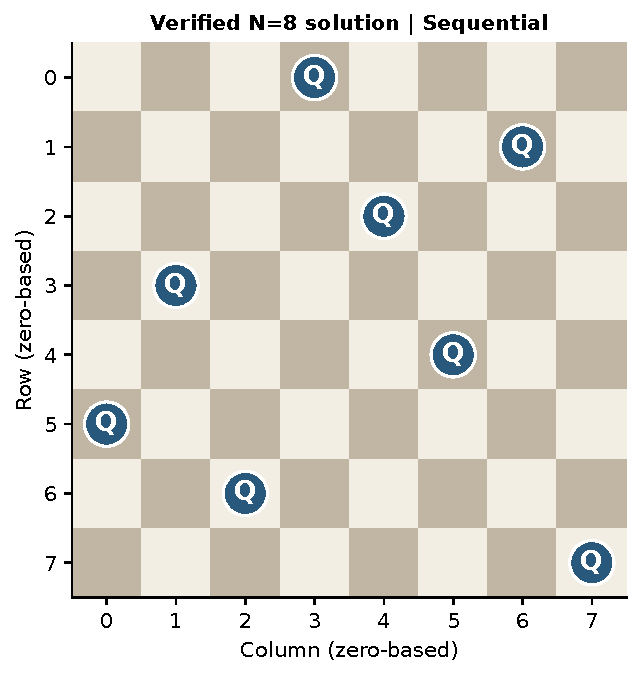
\includegraphics[width=.48\linewidth]{example_board.pdf}
\caption{Một nghiệm $N=8$ lấy từ nhật ký thực nghiệm và kiểm tra độc lập.
Mỗi hàng, cột và đường chéo có nhiều nhất một hậu; có đúng tám hậu.}
\label{fig:board}
\end{figure}

\subsection{Kích thước công thức và ảnh hưởng của mã hóa}

\begin{table}[htbp]
\centering\small
\caption{Kích thước CNF sinh thực tế với $N=128$ trước tiền xử lý}
\label{tab:counts}
\begin{tabular}{lrrrr}
\toprule
Mã hóa & Biến gốc & Biến phụ & Tổng biến & Clause \\
\midrule
Pairwise & 16,384 & 0 & 16,384 & 3,462,784 \\
Binary & 16,384 & 4,854 & 21,238 & 447,832 \\
Sequential & 16,384 & 64,770 & 81,154 & 193,804 \\
Commander & 16,384 & 33,290 & 49,674 & 227,010 \\
Product & 16,384 & 13,798 & 30,182 & 192,906 \\
\bottomrule
\end{tabular}
\end{table}


Các số liệu ở Bảng~\ref{tab:counts} được lấy bằng cách sinh CNF từ cùng mã nguồn
được dùng khi chạy solver. Số biến gồm cả biến bàn cờ và biến phụ; số clause là
số trước tiền xử lý của solver. Pairwise không thêm biến phụ nhưng có tăng trưởng
bậc ba theo $N$. Binary giảm số clause so với pairwise trên bàn lớn và dùng ít biến phụ.
Sequential, commander đệ quy nhóm hằng và product có số clause toàn bàn cờ
$\Theta(N^2)$ với các lựa chọn cụ thể trong báo cáo.

\begin{figure}[htbp]
\centering
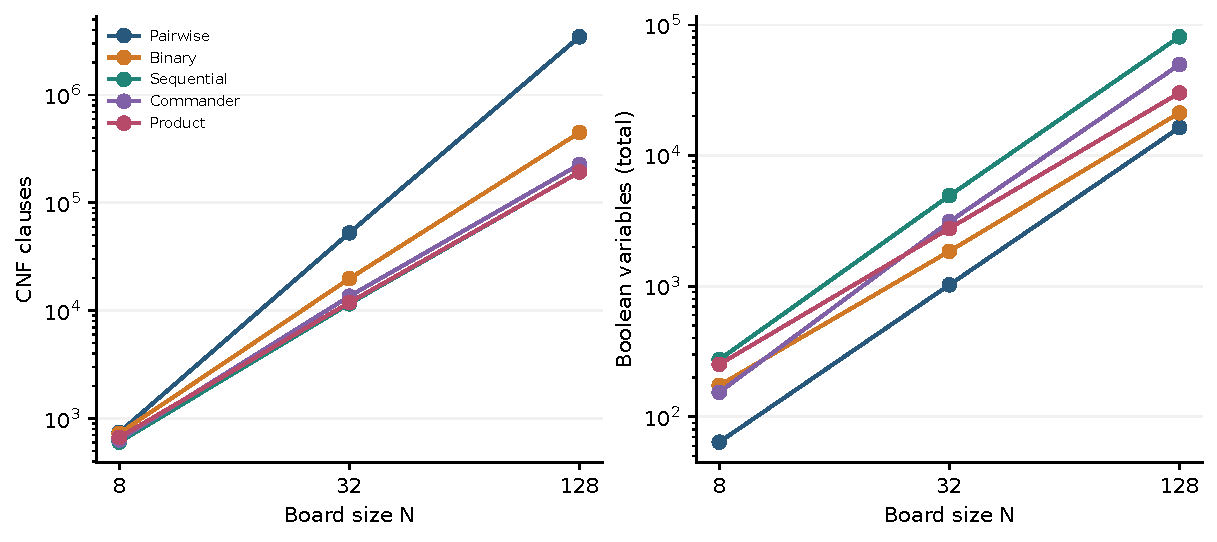
\includegraphics[width=.88\linewidth]{clauses.pdf}
\caption{Số clause trước tiền xử lý của năm mã hóa. Trục tung dùng thang logarit.
Các điểm là số đếm CNF thực tế trên các kích thước được biểu diễn.}
\label{fig:clauses}
\end{figure}

\begin{table}[htbp]
\centering\small
\caption{Thời gian tổng trung vị của SAT trên tập chính tính bằng giây. Mỗi ô số có đủ 3/3 lần SAT; 3 TO nghĩa là cả ba lần hết hạn 30 giây.}
\label{tab:sat}
\FitTableWidth{%
\begin{tabular}{rrrrrr}
\toprule
$N$ & Pairwise & Binary & Sequential & Commander & Product \\
\midrule
8 & 0.000717 & 0.000780 & 0.000674 & 0.000813 & 0.000826 \\
16 & 0.01223 & 0.10084 & 0.008271 & 0.01392 & 0.13646 \\
32 & 0.02734 & 0.06425 & 0.14591 & 0.26885 & 3 TO \\
64 & 0.25442 & 0.06887 & 3 TO & 21.473 & 3 TO \\
128 & 2.405 & 0.34410 & 3 TO & 0.32760 & 0.33250 \\
\bottomrule
\end{tabular}
}
\end{table}


\begin{figure}[htbp]
\centering
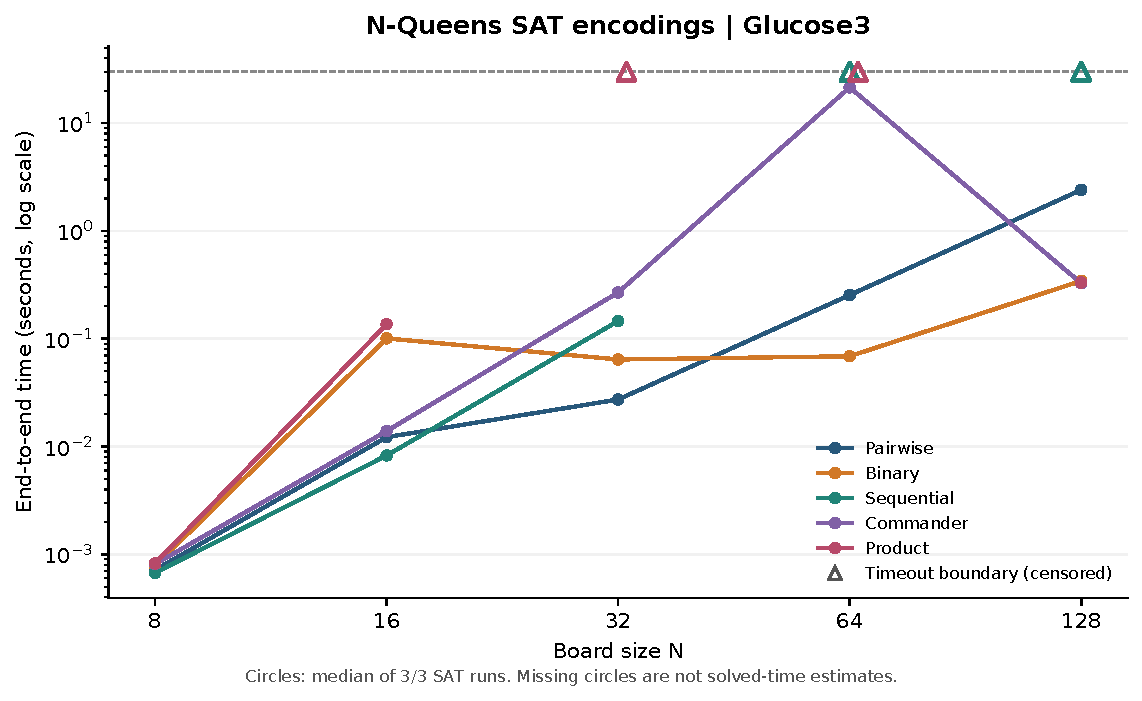
\includegraphics[width=.9\linewidth]{runtime.pdf}
\caption{Thời gian tổng trung vị trên tập chính khi cả ba lần chạy đều thành công.
Dấu hết hạn được đặt ở ngưỡng 30 giây để chỉ giới hạn quan sát, không phải thời gian hoàn thành.}
\label{fig:runtime}
\end{figure}

Trong 75 lần chạy SAT của tập chính, 63 lần tìm được nghiệm đã kiểm tra và 12 lần hết hạn. Ở $N=64$, binary có median 0.0689 giây, trong khi pairwise là 0.2544 giây, tức nhanh hơn khoảng 3.69 lần trong cấu hình này. Sequential và product đều hết hạn ở cả ba lần chạy tại $N=64$. Tại $N=32$, product cũng không hoàn thành trong hạn, dù công thức của nó nhỏ hơn pairwise. Điều đó cho thấy số clause không mô tả đầy đủ cấu trúc lan truyền và tìm kiếm.

Ở $N=128$, pairwise có 3,462,784 clause; product còn 192,906, giảm 94.43\%. Median của binary, commander và product lần lượt là 0.3441, 0.3276, 0.3325 giây. Ba cấu hình này có thời gian gần nhau trên cùng máy; chênh lệch nhỏ không đủ để khẳng định thứ hạng tổng quát. Sequential tiếp tục hết hạn. Commander giảm mạnh thời gian từ $N=64$ sang $N=128$, minh họa tính không đơn điệu của việc tìm một nghiệm trên các kích thước khác nhau.

Tài liệu tham khảo \cite{bach2024} ưu tiên product theo tập chạy của tác giả, nhưng số liệu hiện tại không tái khẳng định một cấu hình luôn thắng. Các kết quả khác nhau có thể liên quan đến quy tắc chia nhóm, công thức cụ thể, thứ tự biến, solver và máy chạy. Báo cáo chỉ quy kết kết quả cho cài đặt và protocol đã công bố, không dùng thời gian trong tài liệu gốc để tính hệ số tăng tốc trên máy hiện tại.

\begin{table}[htbp]
\centering\small
\caption{Các pha thời gian SAT tại $N=128$ tính bằng giây. Mỗi số là trung vị riêng của pha trên ba lần SAT; tổng các trung vị pha không bắt buộc bằng trung vị tổng. TO không có số đo pha hoàn thành.}
\label{tab:phases}
\FitTableWidth{%
\begin{tabular}{lrrrrl}
\toprule
Mã hóa & Tạo CNF & Nạp solver & Tìm nghiệm & Tổng & Nhỏ nhất tới lớn nhất \\
\midrule
Pairwise & 1.3986 & 0.8466 & 0.0316 & 2.4054 & 2.2819--2.4719 \\
Binary & 0.1716 & 0.1217 & 0.0318 & 0.3441 & 0.3418--0.3550 \\
Sequential & -- & -- & -- & TO & -- \\
Commander & 0.0922 & 0.0747 & 0.1453 & 0.3276 & 0.3206--0.3542 \\
Product & 0.0591 & 0.0586 & 0.2008 & 0.3325 & 0.3275--0.3387 \\
\bottomrule
\end{tabular}
}
\end{table}


\subsection{So sánh với CP và MIP}

\begin{table}[htbp]
\centering\small
\caption{So sánh thời gian tổng trung vị tính bằng giây. Best SAT chọn median nhỏ nhất trong các mã hóa đủ 3/3 SAT ở từng N. LIC là giới hạn giấy phép; UNAV là chưa chạy được công cụ.}
\label{tab:compare}
\FitTableWidth{%
\begin{tabular}{rrrrrr}
\toprule
$N$ & Best SAT & CP-SAT & CPLEX MIP & Gurobi & CP Optimizer \\
\midrule
8 & 0.000674 & 0.01068 & 0.006292 & 0.005354 & 0.04959 \\
16 & 0.008271 & 0.01986 & 0.008032 & 0.006576 & 0.04929 \\
32 & 0.02734 & 0.05942 & 3 LIC & 0.01101 & 0.04846 \\
64 & 0.06887 & 0.26568 & 3 LIC & 3 LIC & 0.04713 \\
128 & 0.32760 & 1.504 & 3 LIC & 3 LIC & 0.05566 \\
\bottomrule
\end{tabular}
}
\end{table}

Trên $N=8,16$, CPLEX MIP trả nghiệm hợp lệ trong tất cả các lần chạy; median tại $N=8$ là 0.006292 giây. Từ $N=32$, mô hình có ít nhất 1024 biến nhị phân, vượt mức 1000 biến của bản CPLEX Community đang dùng, nên các ô tương ứng là LIC. CP-SAT và CPLEX CP giải được toàn bộ 15 lần chạy mỗi công cụ trên tập chính. Ở $N=128$, median của CPLEX CP là 0.0557 giây và CP-SAT là 1.5040 giây. Các con số phản ánh cả chi phí mô hình hóa và gọi công cụ trong hai giao diện.

Gurobi giải được cả ba lần tại $N=8,16,32$; median tại $N=32$ là 0.0110 giây. Từ $N=64$, số biến vượt giới hạn 2000 của giấy phép đi kèm nên kết quả là LIC. Trên Windows, giấy phép đi kèm được đặt ở một đường dẫn ASCII để thư viện bản địa đọc được khi thư mục dự án có dấu tiếng Việt. Các lỗi đường dẫn ban đầu được giữ trong \texttt{results/diagnostics} và không được dùng làm thời gian giải. Cột Best SAT thay đổi encoding theo từng kích thước và được chọn sau khi quan sát kết quả; đó là bao dưới thực nghiệm của các cấu hình đã chạy, không phải một bộ chọn encoding được huấn luyện hay một solver mới. Người đọc nên đối chiếu cả Bảng~\ref{tab:sat} để biết phương pháp cụ thể.


\subsection{Khả năng mở rộng và giới hạn nghiên cứu}

\begin{table}[htbp]
\centering\small
\caption{Tập mở rộng với một lần chạy mỗi cấu hình, thời gian tổng tính bằng giây. TO là hết hạn, LIC là giới hạn giấy phép, UNAV là thiếu công cụ hoặc giấy phép, SKIP là vượt trần clause đã định.}
\label{tab:large}
\begin{tabular}{lrrr}
\toprule
Method & 256 & 512 & 1000 \\
\midrule
Pairwise & 1 SKIP & 1 SKIP & 1 SKIP \\
Binary & 2.157 & 7.965 & 1 TO \\
Sequential & 1 TO & 1 TO & 1 TO \\
Commander & 1.225 & 5.508 & 23.900 \\
Product & 1.750 & 3.349 & 14.571 \\
CP-SAT & 15.077 & 1 TO & 1 TO \\
CPLEX MIP & 1 LIC & 1 LIC & 1 LIC \\
Gurobi & 1 LIC & 1 LIC & 1 LIC \\
CP Optimizer & 1 LIC & 1 LIC & 1 LIC \\
\bottomrule
\end{tabular}
\end{table}

Với $N=256$, Binary (2.1575 giây), Commander (1.2245 giây), CP-SAT (15.0771 giây), Product (1.7504 giây) tìm được nghiệm hợp lệ.

Với $N=512$, Binary (7.9649 giây), Commander (5.5075 giây), Product (3.3488 giây) tìm được nghiệm hợp lệ.

Với $N=1000$, Commander (23.9004 giây), Product (14.5712 giây) tìm được nghiệm hợp lệ.

Pairwise ở cả ba kích thước mở rộng vượt trần 5.000.000 clause và được bỏ qua trước khi sinh CNF. Các giới hạn giấy phép được phân biệt với giới hạn thời gian. Mỗi ô ở tập mở rộng chỉ có một lần đo, nên các số này là khảo sát khả năng mở rộng, không cung cấp ước lượng độ biến thiên như tập chính.


Các hạn chế cần được giữ khi diễn giải kết quả. Thứ nhất, chỉ khảo sát bàn cờ trống
và tìm một nghiệm; kết quả không mô tả độ khó của N-Queens Completion hay đếm nghiệm.
Thứ hai, tập kích thước còn hữu hạn và cấu trúc nghiệm thay đổi theo $N$, nên thời gian
không nhất thiết tăng đơn điệu. Thứ ba, ba phép lặp cùng một instance không cho phép
suy rộng thống kê tới mọi bài toán SAT. Thứ tư, giới hạn giấy phép khiến tập so sánh
chung với MIP nhỏ hơn tập SAT/CP; vì thế không dùng các ô bị chặn để khẳng định
một solver chậm hơn. Thứ năm, môi trường máy cá nhân không được cô lập hoàn toàn
khỏi tác vụ hệ thống, nên các chênh lệch rất nhỏ cần được diễn giải thận trọng.
Cuối cùng, báo cáo không xuất chứng chỉ UNSAT để kiểm tra bằng công cụ chứng minh riêng;
các kết luận UNSAT nhỏ được đối chiếu bằng nhiều mã hóa và bộ giải.

\section{Kết luận}
Bài tập đã cài đặt thống nhất năm mã hóa AMO cho N-Queens, xây dựng các mô hình đối chứng CP/MIP và kiểm tra nghiệm độc lập. Bộ kiểm thử xác nhận tính tương đương của AMO trên mọi phép gán nhỏ, trạng thái SAT/UNSAT và số nghiệm của các bàn cờ nhỏ. Thực nghiệm chính cho 63/75 lần SAT thành công, cho thấy binary là lựa chọn thực dụng ở $N=64$ trong cấu hình này, còn các encoding nhỏ về số clause vẫn có thể hết hạn. Ở $N=128$, binary, commander và product có thời gian gần nhau, nên chưa có cơ sở kết luận một encoding luôn tốt nhất.

Khảo sát được thực hiện đến $N=1000$ và kích thước lớn nhất có nghiệm hợp lệ là $N=1000$. Kết quả đối chứng chỉ được so sánh trong miền có dữ liệu chạy hợp lệ; các giới hạn giấy phép được công bố rõ. Hướng tiếp theo là mở rộng giấy phép cho các bộ giải bị giới hạn, tăng số phép lặp trên tập lớn, thử thêm nhiều SAT solver và khảo sát N-Queens Completion bằng cùng cơ chế kiểm tra nghiệm.


\section*{Data Availability}
Mã nguồn, kiểm thử, cấu hình, nhật ký gốc, dữ liệu CSV, script tạo hình và nguồn LaTeX
của bài tập được lưu tại
\url{https://github.com/Duytruong2006/BTL1-NQueens-SAT}.
Bộ bài làm cũng được đóng gói trong tệp \texttt{BTL1\_NguyenDuyTruong\_24021650.zip}.
Repository ở chế độ riêng tư; chủ repository cấp quyền đọc cho giảng viên khi nộp bài.
Các tệp PDF tài liệu môn học và bài báo tham khảo không được phân phối lại trong bộ mã nguồn.

\appendix
\TheorySourceAppendix

\section{Tái lập và đối chiếu yêu cầu}
Các bước tái lập được trình bày trong \texttt{README.md}. Cài đúng phiên bản thư viện
trong \texttt{requirements.txt}, chạy kiểm thử, sau đó chạy hai tập thực nghiệm
bằng \texttt{scripts/benchmark.py}, tổng hợp bằng \texttt{scripts/analyze.py}
và cập nhật báo cáo bằng \texttt{scripts/build\_report.py}.
Script giữ lại nhật ký JSONL trước khi sinh bảng và hình; mỗi nghiệm SAT chứa đủ
danh sách vị trí để người đọc kiểm tra độc lập mà không phải giải lại.
Không xóa các trạng thái lỗi hoặc timeout khỏi mẫu số khi tính tỷ lệ hoàn thành.

\begin{table}[htbp]
\centering\small
\caption{Đối chiếu sản phẩm với yêu cầu Bài tập lớn số 1}
\begin{tabularx}{\linewidth}{p{.31\linewidth}X}
\toprule
Yêu cầu & Sản phẩm và phạm vi đáp ứng\\
\midrule
Cá nhân và chọn N-Queens & Nguyễn Duy Trường, 24021650, CS5; chỉ làm đề tài N-Queens.\\
SAT solver và mã nguồn & Năm encoding CNF; Glucose3 qua PySAT; xuất DIMACS và kiểm tra nghiệm.\\
CPLEX CP, CPLEX MIP, Gurobi, CP-SAT & Đã cài mô hình và chạy công cụ thật; các lần vượt giới hạn giấy phép được công bố riêng.\\
Bàn cờ kích thước lớn & Khảo sát tới $1000\times1000$ trong hạn 30 giây; công bố cả timeout và trường hợp bỏ qua theo trần tài nguyên.\\
Báo cáo dạng bài báo Elsevier & Nguồn LaTeX dùng lớp \texttt{cas-sc}, các bảng và hình sinh từ dữ liệu đo.\\
Data Availability & URL repository thật và gói nguồn kèm kết quả; repository riêng tư cần cấp quyền cho người chấm.\\
\bottomrule
\end{tabularx}
\end{table}

\begin{thebibliography}{99}
\bibitem{bach2024} Trần Ngọc Bách, \emph{An optimized SAT approach solving N-Queens problem},
Technology Project Report, Trường Đại học Công nghệ, ĐHQGHN, 2024. Tài liệu do học phần cung cấp.
\bibitem{module3} Tô Văn Khánh, \emph{At Most One -- AMO, At Least One -- ALO Encoding},
Module3, tài liệu học phần, 17 trang.
\bibitem{module2} Tô Văn Khánh, \emph{SAT Encoding}, Module2, tài liệu học phần, 27 trang.
\bibitem{assignment} \emph{Assignment 1 -- requirements}, Các vấn đề hiện đại KHMT,
HK I năm học 2026--2027, 1 trang.
\bibitem{sample} \emph{Mau xay dung bao cao BTL so 1 và BTL so 2},
bài minh họa \emph{Exact SAT Solving for the Two-Dimensional Bandwidth Minimization Problem},
PDF 32 trang, tài liệu do học phần cung cấp.
\bibitem{pysat} A. Ignatiev, A. Morgado, J. Marques-Silva,
PySAT A Python Toolkit for Prototyping with SAT Oracles, SAT 2018.
\url{https://pysathq.github.io/}.
\bibitem{sinz} C. Sinz, Towards an Optimal CNF Encoding of Boolean Cardinality Constraints,
CP 2005, tr. 827--831. \url{https://www.carstensinz.de/papers/CP-2005.pdf}.
\bibitem{ortools} Google, OR-Tools CP-SAT và mô hình N-Queens,
\url{https://developers.google.com/optimization/cp/queens}.
\bibitem{ibm} IBM, DOcplex và tài liệu CPLEX Python,
\url{https://ibmdecisionoptimization.github.io/docplex-doc/}.
\bibitem{gurobi} Gurobi Optimization, Gurobi Optimizer Reference Manual,
\url{https://docs.gurobi.com/projects/optimizer/en/current/}.
\bibitem{ibmlimits} IBM, CPLEX Optimization Studio Pricing,
\url{https://www.ibm.com/products/ilog-cplex-optimization-studio/pricing}.
\bibitem{gurobilimits} Gurobi, Restricted license for non production use,
\url{https://support.gurobi.com/hc/en-us/articles/29682074018833}.
\bibitem{cas} Elsevier, CAS LaTeX Templates,
\url{https://ctan.org/pkg/els-cas-templates}.
\end{thebibliography}
\end{document}
